%!TEX root = Thesis.tex

\chapter{Lexicon acquisition and annotation}
\label{chap:lexiconAcquisition}
The tiny languages captured by ``handwritten'' lexicons, such as the one demonstrated in the previous chapter, are obviously not a sane option when the grammar is to accept a large vocabulary and a wide range of sentence structures.

In order to use the presented model on a actual data, the acquisition of a wide covering lexicon is crucial. Initially considerable effort was made to \emph{try} to build a CCG lexicon from a \emph{POS-tagged corpus} (part-of-speech-tagged corpus). A POS-tagged corpus is simply a corpus where each token is tagged with a POS-tag, e.g.\ noun, verb, etc. There is no deep structure in such a corpus as opposed to a \emph{treebank}. This approach turned up to have extensive issues as a result of this lack of structure, some of which are detailed in Appendix~\ref{chap:brownCorpus} which succinctly describes the process of the attempt.

There exists some wide covering CCG lexicons, most notable \emph{CCGbank}, compiled by \citeauthor{ccgBank} \shortcite{ccgBank} by techniques presented by \cite{juliaThesis}. It is essentially a translating of almost the entire Penn Treebank \cite{pennTreebank}, which contains over 4.5 million tokens, and where each sentence structure has been analyzed in full and annotated. The result is a highly covering lexicon, with some entries having assigned over 100 different lexical categories. Clearly such lexicons only constitutes half of the previous defined $\mathcal{L}_\textsc{ccg}$ map, i.e.\ only the lexical categories, $\Gamma$. The problem of obtaining a full lexicon, that also yields semantics expressions, is addressed in the next section. It is also worth mentioning that since \citeauthor{baldridgeThesis}'s \shortcite{baldridgeThesis} work on modalities only slightly predates \citeauthor{juliaThesis}'s \shortcite{juliaThesis} work on CCGBank, the CCGBank does not incorporate modalities\footnote{There does exists another project, OpenCCG, started by \citeauthor{baldridgeThesis}, which actually does incorporate modalities, but it has little documentation and was therefore not valued mature enough.}. However more unfortunately is that CCGBank is not free to use, mainly due to license restrictions on the Penn Treebank.% It has not been possible to fund a license.

What might not be as obvious is that besides obtaining a wide-covering lexicon, $\mathcal{L}_\textsc{ccg}$, a even harder problem is for some text $T$ to select the \emph{right} tagging from $\mathcal{L}_\textsc{ccg}(w)$ for each token $w \in T$. \citeauthor{ccgBank} \shortcite{ccgBank} calculate that the expected number of lexical categories per token is 19.2 for the CCGBank. This mean that a exhaustive search of even a short sentence (seven tokens) is expected to consider over 960 million ($19.2^7 \approx \num{961852772}$) possible taggings. This is clearly not a feasible approach, even if the parsing can explore all possible deductions in polynomial time of the number of possible taggings. %, e.g.\ \cite{shiftReduceChart}. 
The number of lexical categories assigned to each token needs to be reduced, however simple reductions as just assigning the most frequent category  observed in some training set (for instance CCGBank) for each token is not a solution. This would fail to accept a large amount of valid sentences, simply because it is missing the correct categories. 

\section{Maximum entropy tagging}
Clearly a solution need to base the reduction on the setting of the token, i.e.\ in which \emph{context} the token appears. \citeauthor{suppertagging} \shortcite{suppertagging} presents a machine learning approach based on a \emph{maximum entropy model} that estimate the probability that a token is to be assigned a particular category, given the \emph{features} of the local context, e.g.\ the POS-tag of the current and adjacent tokens, etc. This is used to select a subset of possible categories for a token, by selecting categories with a probability within a factor of the category with highest probability. \citeauthor{suppertagging} shows that the average number of lexical categories per token can be reduced to 3.8 while the parser still recognize 98.4\% of unseen data. \citeauthor{candc} \shortcite{candc} presents a complete parser, which utilizes this tagging model, and a series of (log-linear) models to speed-up the actual deduction (i.e.\ the parsing) once the tagging model has assigned a set of categories to each token. What maybe even more interesting is that models trained on the full CCGBank, along with toolchain to use them (called the C\&C tools), can be licensed freely for education or research purposes. For this reason it was chosen to use these models and tools.

Furthermore, even though the models neither incorporates modalities, since they are trained on the CCGBank, the deduction models solve many of these problems, since a more plausible deduction (i.e.\ a deduction seen more frequent in the CCGBank) always will suppress other less plausible deductions. Special care are taken about coordination, so neither here seems the lack of modalities to yield significant issues.

\section{Annotating the lexicon}
\label{sec:annotatingLexicon}
The output from the C\&C toolchain can be printed in various formats, including Prolog, which was considered the closest to the presented model, as it, given some set of tokens, $w_1, \ldots, w_n$, simply returns a lexicon and a deduction. An illustrative output for the tokens ``the service was great'' is given in Figure~\ref{fig:candcOutput}. In Chapter~\ref{chap:implementation} more details on the actual format and the processing of it is given.
\begin{figure}[ht]
	\begin{minipage}[b]{0.6\linewidth}
	\center
	\begin{align*}
\alpha_1 &\equiv \mathbf{the} : \mathrm{the}_{\textsc{dt}} \models \cat{NP}_\mathrm{nb} / \cat{N} \\
\alpha_2 &\equiv \mathbf{service} : \mathrm{service}_{\textsc{nn}} \models \cat{N} \\
\alpha_3 &\equiv \mathbf{was} : \mathrm{be}_{\textsc{vbd}} \models (\cat{S}_\mathrm{dcl} \bsl \cat{NP}) / (\cat{S}_\mathrm{adj} \bsl \cat{NP}) \\
\alpha_4 &\equiv \mathbf{great} : \mathrm{great}_{\textsc{jj}} \models \cat{S}_\mathrm{adj} \bsl \cat{NP}
	\end{align*}
	(a) Lexicon
	\end{minipage}
	\hfill
	\begin{minipage}[b]{0.4\linewidth}
	\center
	$$
	  \inference[<]{  
	    \inference[>]{
	      \alpha_1 \;
	      \alpha_2
	    }{
	      \cat{NP}_\mathrm{nb}
	    }
	    \inference[>]{
	      \alpha_3 \;
	      \alpha_4
	    }{
	      \cat{S}_\mathrm{dcl} \bsl \cat{NP}
	    }
	  }{
	    \cat{S}_\mathrm{dcl}
	  }
	$$
	(b) Deduction
	\end{minipage}
	\caption{Illustration of output from the C\&C toolchain.}
	\label{fig:candcOutput}
\end{figure}
\vspace{-1em}

Clearly, deductions in the style previously presented is trivially obtained by substituting the axioms placeholders with the lexicon entries associated. The C\&C toolchain also has a build-in morphological analyzer which allow the lexicon to provide the \emph{lemma} of the tokens and the POS-tag\footnote{Since the C\&C models are trained on CCGBank, which in turn are a translation of The Penn Treebank (PTB), the POS-tag-set used is equivalent to that of PTB cf.\ \cite{pennTreebank}.} of the token. Both of these will be proven convenient later.

There is however one essential component missing from the lexicon, namely the semantic expressions. However due to the \emph{Principle of Categorial Type Transparency} it is known exactly \emph{what} the types of the semantic expressions should be. There are currently a total of 429 different tags in the C\&C tagging model, thus trying to handle each of these cases individually is almost as senseless choice as trying to manually construct the lexicon, and certainly not very robust for changes in the lexical categories. The solution is to handle some cases that need special treatment, and then use a generic annotation algorithm for all other cases. Both the generic and the special case algorithms will be a transformation $(\mathcal{T}, \Sigma^\star) \to \Lambda$, where the first argument is the type, $\tau \in \mathcal{T}$, to construct, and the second argument is the lemma, $\ell \in \Sigma^\star$, of the lexicon entry to annotate. Since the special case algorithms will fallback to the generic approach, in case preconditions for the case are not met, it is convenient to start with the generic algorithm, $\mathcal{U}_\textsc{gen}$, which is given by Definition~\ref{def:Ugen}.

\begin{definition}
	The \emph{generic semantic annotation algorithm}, $\mathcal{U}_\textsc{gen}$ (\ref{eq:Ugen}), for a type $\tau$ and lemma $\ell$ is defined by the auxiliary function $\mathcal{U'}_\textsc{gen}$, which takes two additional arguments, namely an infinite set of variables $\mathcal{V}$ cf.\ Definition \ref{def:Lambda}, and an ordered set of sub-expressions, (denoted $A$), which initially is empty.
\begin{align}
	\mathcal{U}_\textsc{gen}(\tau, \ell) = \mathcal{U}'_\textsc{gen}(\tau, \ell, \mathcal{V}, \emptyset)
	\label{eq:Ugen}
\end{align}

If $\tau$ is primitive, i.e.\ $\tau \in \mathcal{T}_\mathrm{prim}$, then the generic algorithm simply return a functor with name $\ell$, polarity and impact argument both set to $0$, and the ordered set $A$ as arguments. Otherwise there must exists unique values for $\tau_\alpha, \tau_\beta \in \mathcal{T}$, such that $\tau_\alpha \to \tau_\beta = \tau$, and in this case the algorithm return an abstraction of $\tau_\alpha$ on variable $v \in V$, and recursively generates a expression for $\tau_\beta$.
\begin{align*}
	\mathcal{U}'_\textsc{gen}(\tau, \ell,V,A) =
	\begin{cases}
	 \ell_0^0(A) : \tau	&\text{if $\tau \in \mathcal{T}_\mathrm{prim}$} \\	
	 \lambda v . \mathcal{U}'_\textsc{gen}(\tau_\beta, \ell, V \setminus \{v \}, A') : \tau
	&\text{otherwise, where:} %\exists_{\tau_\alpha, \tau_\beta} ( )
	\end{cases}
%	\label{eq:U'gen}
\end{align*}
\begin{align*}
	v &\in V\\
	\tau_\alpha \to \tau_\beta &= \tau\\
	A' &=
	\begin{cases}
    A [e : \tau_\alpha \to \tau_\gamma \mapsto e v : \tau_\gamma ] & \text{if $e' : \tau_\alpha \to \tau_\gamma \in A$} \\ % \tau = \tau_\alpha \to \tau_\beta}  (\tau_\alpha =  \tau_\alpha') \\
    A [e : \tau_\gamma \mapsto v e : \tau_\delta ] & \text{if $\tau_\gamma \to \tau_\delta = \tau_\alpha \wedge e' : \tau_\gamma \in A$}\\
    A \cup \{v : \tau\}) & \text{otherwise}
	\end{cases}
\end{align*}
The recursive call also removes the abstracted variable $v$ from the set of variables, thus avoiding recursive abstractions to use it. The ordered set of sub-expressions, $A$, is modified cf.\ $A'$, where the notation $A[e_1 : \tau_1 \mapsto e_2 : \tau_2]$ is the substitution of all elements in $A$ of type $\tau_1$ with $e_2 : \tau_2$. Note that $e_1$ and $\tau_1$ might be used to determine the new value and type of the substituted elements. Since the two conditions on $A'$ are not mutual exclusive, if both apply the the first case will be selected. The value of $A'$ can be explained in a informal, but possibly easier to understand, manner: 
\begin{itemize}
	\item If there is a least one function in $A$, that takes an argument of type $\tau_\alpha$, then apply $v$ (which is known to by of type $\tau_\alpha$) to all such functions in $A$.
	\item If the type of $v$ itself is a function (i.e.\ $\tau_\gamma \to \tau_\delta = \tau_\alpha$), and $A$ contains at least one element that can be used as argument, then substitute all such arguments in $A$ by applying them to $v$.
	\item Otherwise, simply append $v$ to $A$.
\end{itemize} 
\label{def:Ugen}
\vspace{-1em}
\done
\end{definition}
\clearpage

The get a little familiar with how the generic semantic annotation algorithm works, Example~\ref{ex:Ugen} shows the computation of some types and lemmas.

\begin{example}
	Table~\ref{tabel:Ugen} shows the result of applying $\mathcal{U}_\textsc{gen}\,$on some lemmas and types. The result for a noun as ``room'' is simply the zero-argument functor of the same name. The transitive verb ``provide'' captures two noun phrases, and yields a functor with them as arguments.

	More interesting is the type for the determiner ``every'', when used for instance to modify a performance verb, as shown in Figure~\ref{fig:performanceVerb}. It starts by capturing a noun, then a function over noun phrases, and lastly a noun phrase. The semantic expression generated for this type is a functor, with simply the noun as first argument, and where the second argument is the captured function applied on the noun phrase.

\vspace{1em}
	\begin{table}[!h]
	\begin{center}
	\begin{tabular}{ll|l}
		Lemma & Type & Generic semantic expression \\ \hline		
		&&\\[-8pt]
		room & $\tau_\textsc{n}$ & $\mathrm{room}_0^0$ \\
		provide & $\tau_\textsc{np} \to \tau_\textsc{np} \to \tau_\textsc{s}$ & $\lambda x.\lambda y.\mathrm{provide}_0^0(x, y)$ \\
		every & $\tau_\textsc{n} \to (\tau_\textsc{np} \to \tau_\textsc{s}) \to (\tau_\textsc{np} \to \tau_\textsc{s})$ & $\lambda x.\lambda y.\lambda z.\mathrm{every}_{0}^{0}(x, y\;z)$
	\end{tabular}
	\end{center}
		\caption{Some input/output of generic annotation algorithm}
		\label{tabel:Ugen}
	\end{table}

\vspace{2em}

	\begin{figure}[ht]
	\center
	\scalebox{.7}{
	$
		\inference[<]{\inference{\token{cleaned}\\\pos{VBN}}{\cat{S}_\mathrm{pss} \bsl \cat{NP}_{}:\lambda x.\mathrm{clean}_{0}^{0}(x)}\inference[>]{\inference{\token{every}\\\pos{DT}}{((\cat{S}_{x} \bsl \cat{NP}_{}) \bsl (\cat{S}_{x} \bsl \cat{NP}_{}))/\cat{N}_{}:\lambda x.\lambda y.\lambda z.\mathrm{every}_{0}^{0}(x, y\;z)}\inference{\token{day}\\\pos{NN}}{\cat{N}_{}:\mathrm{day}_{0}}}{(\cat{S}_{x} \bsl \cat{NP}_{}) \bsl (\cat{S}_{x} \bsl \cat{NP}_{}):\lambda y.\lambda z.\mathrm{every}_{0}^{0}(\mathrm{day}_{0.0}, y\;z)}}{\cat{S}_\mathrm{pss} \bsl \cat{NP}_{}:\lambda z.\mathrm{every}_{0}^{0}(\mathrm{day}_{0}, \mathrm{clean}_{0}^{0}(z))}
	$
	}
	\caption{Complex determiner modifying performance verb.}
	\label{fig:performanceVerb}
	\end{figure}
	\label{ex:Ugen}
	
\end{example}
\done
\vspace{1em}

Clearly the generic algorithm does not provide much use with respect to extracting the sentiment of entities in the text, i.e.\ it only provide some safe structures that are guaranteed to have the correct type. The more interesting annotation is actually handled by the special case algorithms. How this is done is determined by a combination of the POS-tag and the category of the entry. Most of these treatments are very simple, with the handling of adjectives and adverbs being the most interesting. The following briefly goes through each of the special case annotations.

\begin{itemize}
	\item \emph{Determiners} with simple category, i.e.\ $\cat{NP}/\cat{N}$, are simply mapped to the identity function, $\lambda x.x$.
	While determiners have high focus in other NLP tasks, such as determine if a sentence is valid, the importance does not seem significant in sentiment analysis, e.g.\ whether an opinion is stated about \emph{some} or \emph{all} of entities does not change the overall polarity of the opinion bound to that entity.

	\item \emph{Nouns} are in general just handled by the generic algorithm, however in some cases of multi-word nouns, the sub-lexical entities may be tagged with the category $\cat{N}/\cat{N}$. In these cases the partial noun is annotated with a list structure, that eventually will capture the entire noun, i.e.\ $\lambda x.\langle \mathcal{U}_\textsc{gen}(\tau_\textsc{n}, \ell), x\rangle$, where $\ell$ is the lemma of the entity to annotate.

	\item \emph{Verbs} are just as nouns in general handled by the generic algorithm, however \emph{linking verbs} are a special case, since they relate the subject (i.e.\ a entity) with one or more \emph{predicative adjectives}. Linking verbs have the category $(\cat{S}_\mathrm{dcl} \bsl \cat{NP})/(\cat{S}_\mathrm{adj} \bsl \cat{NP})$, and since the linked adjectives directly describes the subject of the phrase such verbs are simply annotated with the identity function, $\lambda x.x$. 

	\item \emph{Adjectives} can have a series of different categories depending on how they participate in the sentence, however most of them have the type $\tau_\alpha \to \tau_\beta$, where $\tau_\alpha, \tau_\beta \in \mathcal{T}_\mathrm{prim}$. These are annotated with the \emph{change} of the argument, i.e. $\lambda x.x_{\circ j}$, where $j$ is a value determined based on the lemma of the adjective. Notice that this assumes implicit type conversion of the parameter from $\tau_\alpha$ to $\tau_\beta$, however since these are both primitive, this is a sane type cast. Details on how the value $j$ is calculated are given in Section~\ref{sec:sentimentAdj}.

	\item \emph{Adverbs} are annotated in a fashion closely related to that of adjectives. However the result might either by a \emph{change} or a \emph{scale}, a choice determined by the lemma: normally adverbs are annotated by the change in the same manner as adjectives, however \emph{intensifiers} and \emph{qualifiers}, i.e.\ adverbs that respectively strengthens or weakens the meaning, are scaled. Section~\ref{sec:sentimentAdverb} gives further details on how this choice is made. Finally special care are taken about negating adverbs, i.e. ``not'', which are scaled with a value $j = -1$.

	\item \emph{Prepositions} and \emph{relative pronouns} need to change the impact argument of captured partial sentences, i.e.\ \emph{preposition phrases} and \emph{relative clauses}, such that further modification should bind to the subject of the entire phrase as were illustrated by Example~\ref{ex:semantics2}.

	\item \emph{Conjunctions} are annotated by an algorithm closely similar to $\mathcal{U}_\textsc{gen}$, however instead of yielding a functor of argument, the algorithm yields a list structure. This allow any modification to bind on each of the conjugated sub-phrases.
	
\end{itemize}


\section{Semantic networks}
\label{sec:sentimentValue}

In order to reason about the polarity of the entities present in the text to analyse, a understanding of the domain of the review is needed.  For this purpose the concept of \emph{semantic networks} is introduced. Formally a semantic network is a structure cf.\ Definition~\ref{def:SemanticNetwork}.
\begin{definition}
a semantic network is a quadruple $(L,S,R,M)$ where:\\[-2em]
  \begin{itemize} %[labelindent=2em,labelwidth=0em,itemindent=0em,leftmargin=2em]
    \item $L \subset \Sigma^\star$ is the set of lexical units recognized by the network.
    \item $S$ is the set of \emph{semantic concepts} in the network.
    \item $R$ is a set of binary relations on $S$ where the relation $r \in R$ describes links\\ between semantic concepts, i.e.\ $r \subset S \times S$. 
    \item $M$ is a mapping from lexical units to a set of semantic entities that the lexical\\ unit can entail, i.e.\ $M: L \to \mathcal{P}(S)$.
  \end{itemize}
  \label{def:SemanticNetwork}
  \vspace{-1em}
  \done
\end{definition}
\vspace{-2em}

Notice that $S$ and $R$ constitutes a set of graphs, i.e.\ for each relation $r \in R$ the graph~$(S,r)$. The graph is undirected if $r$ is \emph{symmetric}, and directed if $r$ is \emph{asymmetric}. An illustrative example of such a graph, denoting a relation in a extract of a semantic network of adjective concepts is given in Figure~\ref{fig:semanticNetwork}.  Since a lexical unit might entail many different concepts cf.\ Definition~\ref{def:SemanticNetwork}, semantic concepts is described by the set of lexical unit that can entail it, each denoted with the index that uniquely identifies that meaning of the lexical unit. For instance in Figure~\ref{fig:semanticNetwork} the 4th meaning of \emph{olympian} entail the same semantic concept as the 1st meaning of \emph{exceptional}.

\begin{figure}[ht]
  \center
  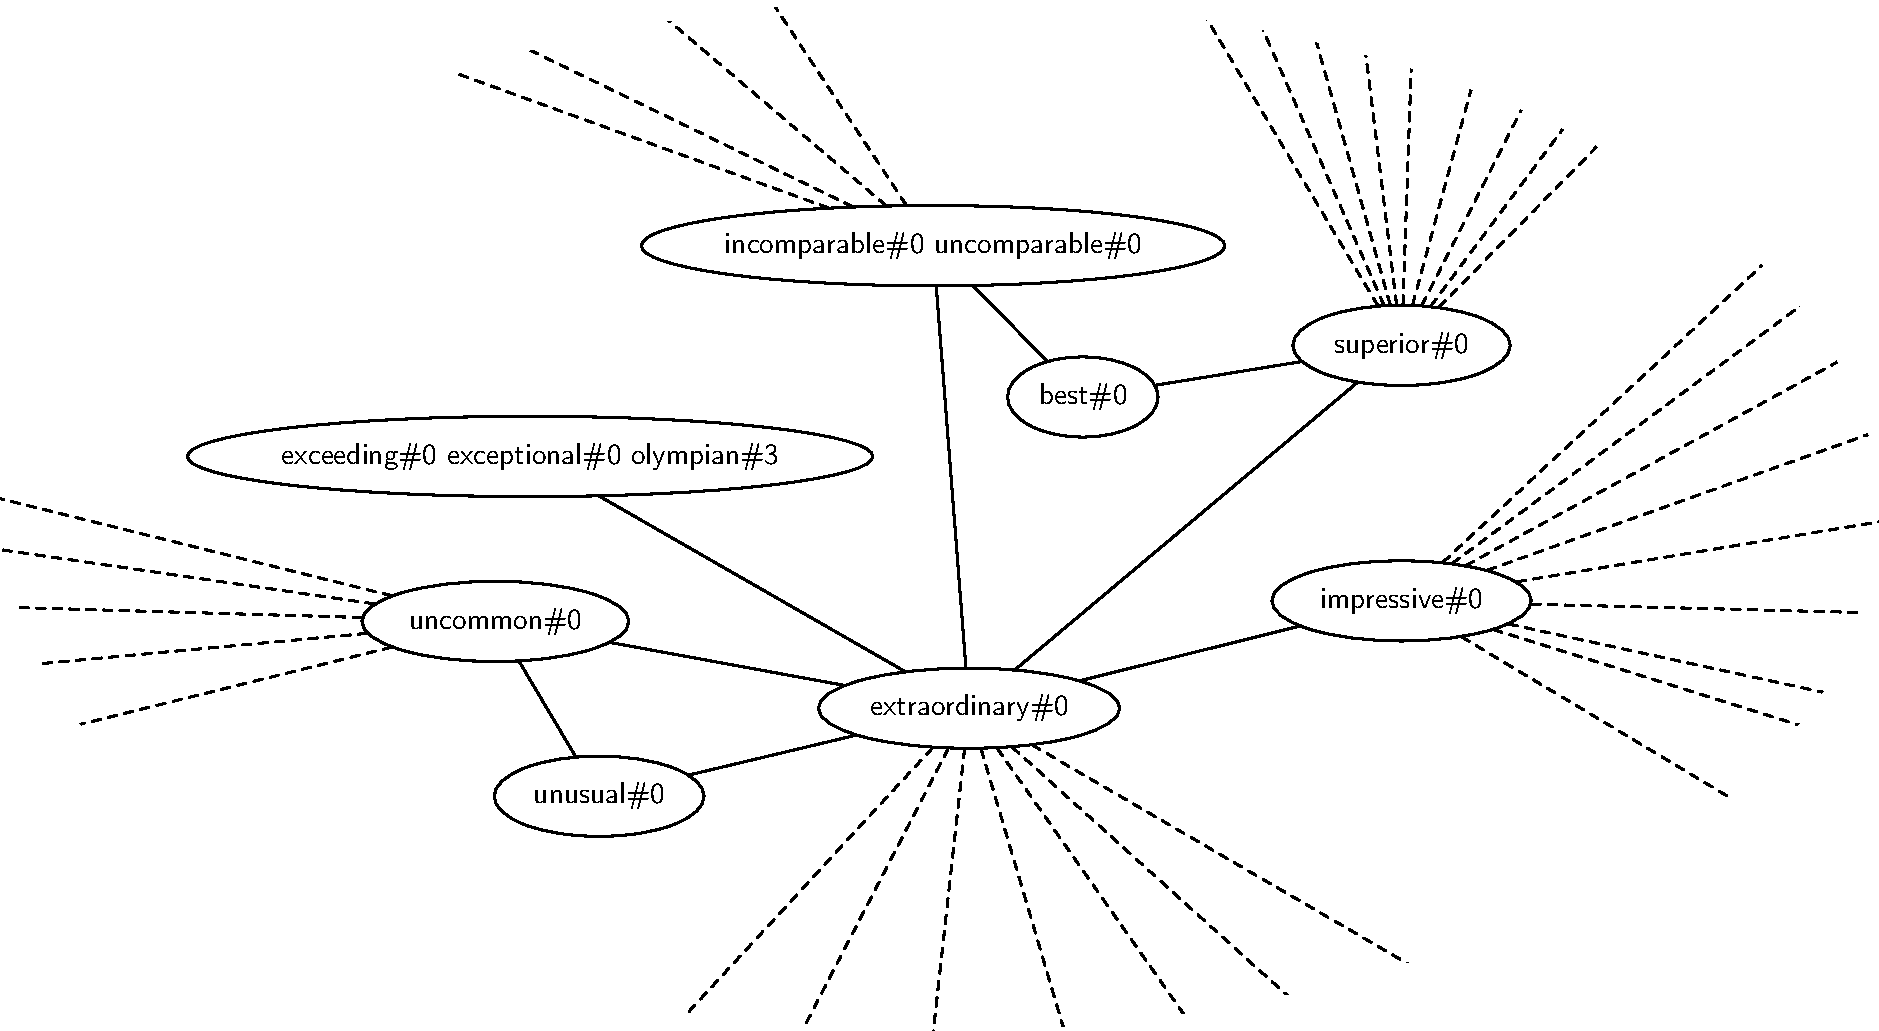
\includegraphics[scale=.27]{Figures/Exceptional}
  \caption{Illustration of relation in a semantic network.}
  \label{fig:semanticNetwork}
\end{figure}

The concrete semantic network used is WordNet, originally presented by \citeauthor{wordnet} \shortcite{wordnet}, and later presented in depth by \citeauthor{wordnetBook} \shortcite{wordnetBook}. Like it was the issue when acquiring a lexicon for the syntactic analysis, the availability of free semantic networks is very sparse. It has not been possible to find other competing networks with a coverage close to that of WordNet, and thus the decision of using WordNet is really based on it being the only choice. With that said, it is argued that WordNet is a quite extensive semantic network, which in its most recent revision (3.0) contains a relatively large number of semantic concepts, namely $|S| \approx \num{117000}$, while the number of lexical units recognized may be argued is not as covering as ideally, namely $|L| \approx \num{155000}$.

WordNet contains a variety of relations, $R$, however for the purpose of calculating sentiment polarity values, only the following were considered interesting:
\begin{itemize}
	\item The \emph{similar}-relation, $r_\mathrm{similar}$, links \emph{closely similar} semantic concepts, i.e.\ concepts having almost the synonymies mensing in most contexts. The relation is present for most concepts entailed by adjectives.
	\item The \emph{see also}-relation, $r_\mathrm{see\text{-}also}$, links \emph{coarsely similar} semantic concepts, i.e.\ concepts having a clear different mensing, but may be interpreted interchangeably for some contexts. Figure~\vref{fig:semanticNetwork} shows an example of exactly the \emph{see also}-relation.
	\item The \emph{pertainym}-relation, $r_\mathrm{pertainym}$, links the adjectives from which a adverb was derived, e.g.\ \emph{extreme} is the pertainym of \emph{extremely}.
\end{itemize}
\vspace{1em}

\section{Sentiment polarity of adjectives}
\label{sec:sentimentAdj}
The approach used to calculate sentiment polarity values for adjectives is very similar to the one presented by \citeauthor{valenceShifting} \shortcite{valenceShifting}, namely a domain specific set of positive and negative \emph{seed concepts} are identified, respectively $S_\mathrm{pos}$ and $S_\mathrm{neg}$. Each semantic concept in the sets can be described by a lexical unit and the specific index for that lexical unit that entail the desired concept, e.g.\ as shown in (\ref{eq:s_pos}) and (\ref{eq:s_neg}).
\begin{align}
	S_\mathrm{pos} &= \left\{ \text{clean}\#1, \text{quiet}\#1, \text{friendly}\#1, \text{cheap}\#1 \right\} \label{eq:s_pos}\\
	S_\mathrm{neg} &= \left\{ \text{dirty}\#1, \text{noisy}\#1, \text{unfriendly}\#1, \text{expensive}\#1 \right\} \label{eq:s_neg}
\end{align}

The graph $G_\mathrm{adj}$, given by (\ref{eq:g_adj}), is considered to calculate the sentiment polarity change inflicted by the adjective. Notice that the graph includes both the \emph{similar}-relation and the \emph{see\ also}-relation, as is desired to be able to reason about as large a set of adjectives as possible, and thus both closely and coarsely related concepts are considered.
\begin{align}
	G_\mathrm{adj} = (S, r_\mathrm{similar} \cup r_\mathrm{see\text{-}also})
	\label{eq:g_adj}
\end{align}
 
Given an adjective with lemma $\ell \in \Sigma^\star$, the set of semantic concepts that this adjective may entail, $M(\ell)$, should provide the basis for the sentiment polarity change inflicted by the adjective. The overall approach is to base the polarity change on the \emph{distances} between the concepts yielded by $M(\ell)$ and the seed concepts in $G_\mathrm{adj}$. However, as the system only has very limited domain knowledge, namely $S_\mathrm{pos}$ and $S_\mathrm{neg}$, there are no sure way of choosing which of the semantic concepts yielded by $M(\ell)$ is the ``right'' interpretation of $\ell$. Considering all of the possible concepts yielded by $M(\ell)$ nigher seem like a sane choice, since this would evidently flatten the polarities and end in vague results. The method used to solve this semantic ambiguity follows from the rational assumption that adjectives stated in the texts presumably are to be interpreted within the domain given by the seed concepts. Thus concepts from $M(\ell)$ that are strongly related to one or more seed concepts should be preferred over weaklier related concepts. The solution is to select the $n$ \emph{closest} relations between $M(\ell)$ and respectively $S_\mathrm{pos}$ and $S_\mathrm{neg}$, thus reasoning greedily positively, respectively greedily negatively, about $\ell$. The \emph{multiset} of all distances to either seed set for some lemma $\ell$ is given by $D_\mathrm{adj}(\ell, S')$, where $S'$ is either $S_\mathrm{pos}$ or $S_\mathrm{neg}$ cf.\ (\ref{eq:dist_adj}), and where $d_\mathrm{adj}$ is the distance function for $G_\mathrm{adj}$. The sub-multiset of $D_\mathrm{adj}(\ell, S')$ which contains the minimal $n$ values is denoted $D^n_\mathrm{adj}(\ell, S')$.
\begin{align}
    D_\mathrm{adj}(\ell, S') = \left[ d_\mathrm{adj}(s, s') \; | \; s \in M(\ell), s' \in S' \right] & \hspace{2em} \text{where $S' \in \{ S_\mathrm{pos}, S_\mathrm{neg}$ \}}
	\label{eq:dist_adj}
\end{align}

Finally the sentiment polarity for an adjective with lemma $\ell$, denoted $p_\mathrm{adj}(\ell)$, is then given by the \emph{difference} of the sums of the $n$ minimal \emph{normalized distances} cf.\ (\ref{eq:p_adj}), where $N$ is a normalization factor, ensuring that $p_\mathrm{adj}(\ell) \in \left[-\omega; \omega \right]$. This follows the intuition, that positive adjectives are \emph{closer} to $S_\mathrm{pos}$ than $S_\mathrm{neg}$ and vice-verse.
\begin{align}
    p_\mathrm{adj}(\ell) =     	
    	\left( \sum_{j \in  D^n_\mathrm{adj}(\ell, S_\mathrm{neg}) } N \cdot j \right) -
		\left( \sum_{j \in  D^n_\mathrm{adj}(\ell, S_\mathrm{pos}) } N \cdot j \right)
	\label{eq:p_adj}
\end{align}

Clearly this intuition is only valid if $|S_\mathrm{pos}| \approx |S_\mathrm{neg}|$, or more precisely, the probability of some random semantic concept is close to a positive concept should be the same as the probability of it being close to a negative concept. %Furthermore it is assumed that $d_\mathrm{adj}$ is \emph{normalized} cf.\ (\ref{eq:d_adj}), i.e. it always yields a value, such that $p_\mathrm{adj}(\ell) \in \left[-\omega; \omega \right]$.
%\begin{align}
%    d_\mathrm{adj}(s, s') \in \left[0; \frac{\omega}{n \cdot k}\right]	&\hspace{4em} \text{where $k = |S_\mathrm{pos}| = |S_\mathrm{neg}|$}
%    \label{eq:d_adj}
%\end{align}

The semantic expression of an adverb with type $\tau_\alpha \to \tau_\alpha$ is given by $e_\mathrm{adj}(\ell)$ in (\ref{eq:e_adj}).
\begin{align}
	e_\mathrm{adj}(\ell) &=
    \lambda x . x_{\circ p_\mathrm{adj}(\ell)}
	\label{eq:e_adj}
\end{align}

The calculation of $p_\mathrm{adj}(\ell)$ can be generalized for any semantic graph $G$, given its distance function $d$, and sets of respectively positive and negative \emph{seed concepts} $S_\mathrm{p}$ and $S_\mathrm{n}$ cf.\ (\ref{eq:p}). This generalization will be convenient in a moment, and $p_\mathrm{adj}$ is trivially expressible in terms of $p$: $p_\mathrm{adj}(\ell) = N \cdot p(d_\mathrm{adj}, S_\mathrm{pos}, S_\mathrm{neg}, \ell)$.
\begin{align}
    p(d, S_\mathrm{p}, S_\mathrm{n}, \ell) =     	
    	\left( \sum_{j \in  D_d^n(\ell, S_\mathrm{n}) } j \right) -
		\left( \sum_{j \in  D_d^n(\ell, S_\mathrm{p}) } j \right)	
	\label{eq:p}
\end{align}
where:
\begin{align}
	D_d(\ell, S') = \left[ d(s, s') \; | \; s \in M(\ell), s' \in S' \right] 
	\label{eq:p}
\end{align}

%The sentiment polarity for an adjective with lemma $\ell$ is denoted $p(G, S_\mathrm{pos}, S_\mathrm{neg}, \ell)$, where $G$ is the semantic graph, and $S_\mathrm{pos}, S_\mathrm{neg}$ are  cf.\ (\ref{eq:p_dcl})

\section{Sentiment polarity of adverbs}
\label{sec:sentimentAdverb}
The approach for calculating sentiment polarity values for adverbs is very similar to the approach used for adjectives. In fact, since WordNet does not define neither $r_\mathrm{similar}$ nor $r_\mathrm{see\text{-}also}$ on adverbs the basic approach is simply to lookup the adjective from which the adverb is derived from, if any, using $r_\mathrm{pertainym}$. However since adverbs might also \emph{intensify} or \emph{qualify} the meaning of a verb, adjective, or another adverb, some special treatment are presented for this. Analog to the positive and negative concepts, sets of respectively intensifying and qualifying seed adjectives are stated, e.g.\ (\ref{eq:s_itensify}) and (\ref{eq:s_qualify}).
\todo{Rethink those?}
\begin{align}
	S_\mathrm{intensify} &= \left\{ \text{extreme}\#1, \text{much}\#1, \text{more}\#1)\right\} \label{eq:s_itensify}\\
	S_\mathrm{qualify} &= \left\{ \text{moderate}\#1, \text{little}\#1, \text{less}\#1) \right\} \label{eq:s_qualify}
\end{align}

Recall from Section~\ref{sec:annotatingLexicon} that intensifiers and qualifiers are \emph{scaling} the value of the verb, adjective or adverb they modify. To calculate the factor of which an intensifier or qualifier inflicts, the graph $G_\mathrm{scale}$, given by (\ref{eq:g_scale}), is considered. The graph only contains the \emph{similar}-relation, since related intensifiers, respectively qualifiers, seem to be captured most precisely by only considering \emph{closely similar} adjectives to the selected seeds cf.\ \cite{valenceShifting}. Also notice that, unlike $S_\mathrm{pos}$ and $S_\mathrm{neg}$, these sets does not rely on the domain, as they only strengthens or weakens domain specific polarities. 
\begin{align}
	G_\mathrm{scale} = (S, r_\mathrm{similar})
	\label{eq:g_scale}
\end{align}

%The distance function for $G_\mathrm{scale}$, denoted $d_\mathrm{scale}$ is normalized such that the polarity of the adverb is in the range $[-1; 1]$ cf.\ (\ref{eq:d_scale}).
%\begin{align}
%    d_\mathrm{scale}(s, s') \in \left[0; \frac{1}{n \cdot k}\right]	&\hspace{4em} \text{where $k = |S_\mathrm{intensify}| = |S_\mathrm{qualify}|$}
%    \label{eq:d_scale}
%\end{align}

The value of a polarity scaling is then given by the exponential function (\ref{eq:p_scale}) with range $\left[\frac{1}{2}; 2 \right]$, i.e. the value of $p(d_\mathrm{scale}, S_\mathrm{intensify}, S_\mathrm{qualify}, \ell)$ is normalized using $N$ such it yields the range $[-1; 1]$. Thus a strong intensifier can double the sentiment polarity value of the unit it modifies, analogously a strong qualifier can reduce it by half.  
\begin{align}
    p_\mathrm{scale}(\ell) = 2^{N \cdot p(d_\mathrm{scale}, S_\mathrm{intensify}, S_\mathrm{qualify}, \ell)}
    \label{eq:p_scale}
\end{align}

Whether an adverb is considered and intensifier/qualifier or an normal adverb is determined by the value of $p_\mathrm{scale}(\ell')$, where $\ell'$ is the pertainym of the adverb. The semantic expression of an adverb with type $\tau_\alpha \to \tau_\alpha$ is given by $e_\mathrm{adverb}(\ell)$ in (\ref{eq:e_adverb}). If $p_\mathrm{scale}(\ell') \neq 1$ then the adverb is considered as a intensifier/qualifier and scales the lexical unit it inflicts, otherwise if the adverb is an derivation of an adjective it simply changes the inflicted unit with the value of the adjective. Finally the adverb can be one of a small set of predefined negatives, $L_\mathrm{neg}$, in this case the polarity of the inflicted unit is flipped. Otherwise the adverb is discarded by simply being annotated with the identity function.
\begin{align}
	e_\mathrm{adverb}(\ell) &=
	\begin{cases}    
    \lambda x . x_{\bullet p_\mathrm{scale}(\ell')} & \text{if $M(\ell) \times M(\ell') \subset r_\mathrm{pertainym}$ and $p_\mathrm{scale}(\ell') \neq 1$} \\
    \lambda x . x_{\circ p_\mathrm{adj}(\ell')} & \text{if $M(\ell) \times M(\ell') \subset r_\mathrm{pertainym}$} \\
    \lambda x . x_{\bullet -1} & \text{if $\ell \in L_\mathrm{neg}$}\\
    \lambda x . x & \text{otherwise}
	\end{cases}
	\label{eq:e_adverb}
\end{align}

\section{Completing the analysis}
All the components needed in order to calculate the sentiment of a text 
  \begin{align}
	 \mathcal{A}: \Sigma^\star \to S \to [-\omega;\omega] \tag{\ref{eq:Analysis}}	 
  \end{align}
% with the obvious exception that the distance function used of cause is with respect to $G_\mathrm{scale}$, and not $G_\mathrm{adj}$.